%%%%%%
%
% $Autor: Wings $
% $Datum: 2020-01-18 11:15:45Z $
% $Pfad: githubtemplate/Template/Presentations/Template/slides/rename.tex $
% $Version: 4620 $
%
%
% !TeX encoding = utf8
% !TeX root = Rename
%
%%%%%%



\Mysection{NVIDIA Jetson Nano Developer Kit}
\STANDARD{NVIDIA Jetson Nano Developer Kit}
{
The \textbf{NVIDIA Jetson Nano Developer Kit} is a compact and powerful embedded computing platform
designed for edge AI and robotics. It enables developers to run multiple neural networks in parallel
for tasks such as object detection, segmentation, and speech processing.\cite{NVIDIA:2020}

\pagebreak
	\begin{figure}
		\centering 
		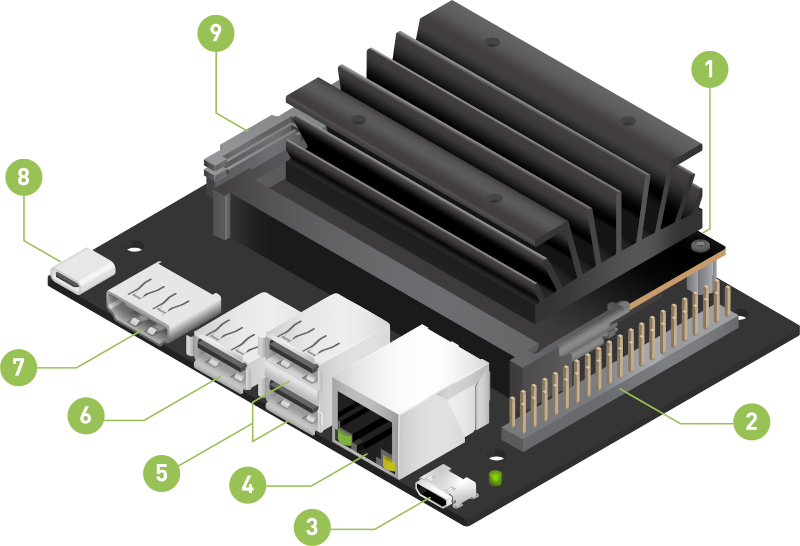
\includegraphics[width=0.5\linewidth]{../NVIDIAJetsonNano/images/JetsonN.png}
		\caption{NVIDIA Jetson Nano Developer Kit\cite{NVIDIA:2020b} \linebreak	1. microSD card slot for main storage,
		2.	40-pin expansion header,
		3.	Micro-USB port for Device Mode,\linebreak
		4.	Gigabit Ethernet port,
		5.	USB 2.0 ports (x2),
		6.	USB 3.0 port (x1),\linebreak
		7.	HDMI output port,
		8.	USB-C for 5V power input,
		9.	MIPI CSI-2 camera connector
		 }
	\end{figure}
	

}

\STANDARD{Key Features}
{
\begin{itemize}
	\item GPU-accelerated edge computing with low power consumption.
	\item Full Linux (Ubuntu-based) development environment.
	\item Support for NVIDIA JetPack SDK and TensorRT.
	\item Compatible with many open-source AI frameworks such as TensorFlow, PyTorch, and OpenCV.
\end{itemize}
}
% ---- DATASHEET REFERENCE ----
\Mysection{Datasheet Reference}

\STANDARD{Official Reference}
{
For full specifications and design information, refer to the official NVIDIA datasheet:

\begin{itemize}
	\item NVIDIA Corporation, \textit{NVIDIA Jetson Nano Developer Kit — Data Sheet}, Version 1.1, 2020.
	\item Available at: \href{https://developer.nvidia.com/embedded/jetson-nano}{Developer Kit}
\end{itemize}
}

% ---- HARDWARE SPECIFICATIONS ----
\Mysection{Hardware Specifications}

\STANDARD{Core Hardware}
{
\begin{itemize}
	\item \textbf{GPU:} 128-core NVIDIA Maxwell architecture.
	\item \textbf{CPU:} Quad-core ARM Cortex-A57 @ 1.43 GHz.
	\item \textbf{Memory:} 4 GB 64-bit LPDDR4 @ 25.6 GB/s.
	\item \textbf{Storage:} microSD card slot for system and user data.
	\item \textbf{Networking:} Gigabit Ethernet (10/100/1000 BASE-T).
	\item \textbf{Display:} HDMI 2.0 / DP 1.2, up to 4K @ 60 Hz.
	\item \textbf{Camera:} MIPI CSI-2 x2 interfaces.
	\item \textbf{Video Encode:} 4K @ 30 fps (H.264/H.265).
	\item \textbf{Video Decode:} 4K @ 60 fps (H.264/H.265).
	\item \textbf{I/O:} 40-pin GPIO header (I\textsuperscript{2}C, SPI, UART, I\textsuperscript{2}S, GPIO).
	\item \textbf{Power:} 5 V DC (micro-USB or barrel jack input).
\end{itemize}
\pagebreak
\textbf{Power Modes}
\begin{itemize}
	\item 5 W power mode for low-power applications.
	\item 10 W mode for high-performance workloads.
\end{itemize}
}

\STANDARD{NVIDIA Jetson Nano Developer Kit Carrier Board}
{
	\begin{figure}
	\centering 
	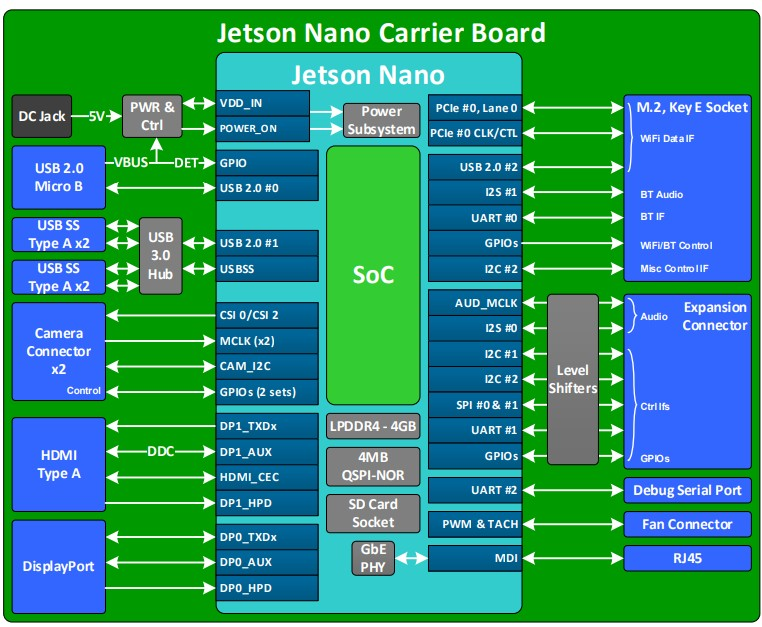
\includegraphics[width=0.5\linewidth]{../NVIDIAJetsonNano/images/JetsonNCB.jpg}
	\caption{NVIDIA Jetson Nano Developer Kit Carrier Board\cite{NVIDIA:2020b} }
	\end{figure}
}


\Mysection{Sensors in NVIDIA Jetson Nano Developer Kit}
\STANDARD{Sensors in NVIDIA Jetson Nano Developer Kit}
{
The Jetson Nano supports a variety of sensor interfaces (e.g., I²C, SPI, UART, GPIO) enabling connection of many sensors for e.g.\ temperature, humidity, motion, proximity. According to Kurniawan (2021) it “can implement IoT solutions … with the board having GPIO pins and a GPU core”.  
Although specific sensor modules are external, typical sensors used with Jetson Nano include IMUs, LiDARs, ultrasonic distance sensors, environmental sensors, etc. For these sensors you would write code to interface over I²C/SPI or via USB.
}

\Mysection{Testing codes for all the sensors}
\STANDARD{Testing codes for all the sensors}
{
After connecting sensors to Jetson Nano, you would write test code. For example, using Python with libraries such as 
\texttt{smbus2} for I²C, \texttt{spidev} for SPI, \texttt{serial} for UART, and GPIO via \texttt{Jetson.GPIO}. Micro-example:  
	\lstinputlisting[language=Python,style=mystyle,firstline=1,firstnumber=1]{Code/Tests.py}


You would test each sensor: initialise it, read raw values, process/validate them, log results. For IoT sensor-reading with Jetson Nano see e.g.\ the study on agricultural machines: “Engineering of Information Monitoring System Sensor Reading Data Based on Smart Wireless using NVIDIA Jetson Nano and Arduino Mega…” 
}

\Mysection{Compatible Camera for NVIDIA Jetson Nano Developer Kit}
\STANDARD{Compatible Camera for NVIDIA Jetson Nano Developer Kit}
{
The Jetson Nano supports MIPI CSI-2 camera modules (2 lanes) and USB cameras. The book by Kurniawan (2021) mentions “the board … enable[s] stronger IoT solutions … with integrated sensor and actuators” and includes a chapter on the camera.  When selecting a camera ensure driver support under the OS and suitable resolution/frame rate for your application (e.g., 1080p @30 fps or better for real-time vision).  
}

\Mysection{OS compatible with NVIDIA Jetson Nano Developer Kit}
\STANDARD{OS compatibility}
{
The NVIDIA Jetson Nano Developer Kit officially uses the NVIDIA JetPack SDK (which includes Ubuntu Linux, CUDA, cuDNN, TensorRT). 
According to NVIDIA Jetson Nano Datasheet, you can install Ubuntu 18.04/20.04 based images provided by NVIDIA. Some community builds support other Linux distributions but for full GPU/vision support JetPack is recommended.
}

\Mysection{OS installation in NVIDIA Jetson Nano Developer Kit}
\STANDARD{OS Installation}
{
Here is a high-level installation process:  
\begin{itemize}
\item Download the JetPack image from NVIDIA’s website.
\item Flash the microSD card (or eMMC/module depending variant) with the image.
\item Insert into Jetson Nano, connect keyboard/monitor, power it up.
\item Follow on-screen initial setup (locale, timezone, user, WiFi/Ethernet).
\item Run the SDK Manager or apt-install additional packages (CUDA, cuDNN, TensorRT).
\end{itemize}
}

\Mysection{Setup after OS Installation in NVIDIA Jetson Nano Developer Kit}
\STANDARD{Setup after OS Installation}
{
After OS installation you should perform:  
\begin{itemize}
\item Update and upgrade the system: \texttt{sudo apt update \&\& sudo apt upgrade}.
\item Enable necessary services (e.g., ssh, VNC).
\item Test GPU/CUDA: run \texttt{nvidia-smi} or the Jetson Stats tool.
\item Install camera drivers and verify camera input (e.g., \texttt{gst-launch-1.0} for CSI camera).
\item Configure sensor interfaces: enable I²C, SPI in device tree or via \texttt{/boot/firmware/config.txt} if needed.
\item Clone/test sample code (e.g., for object detection) — many papers show such usage: see e.g.\ “Benchmarking Deep Learning Models on NVIDIA Jetson Nano”
\end{itemize}
}

\Mysection{Connector cables compatible with NVIDIA Jetson Nano Developer Kit}
\STANDARD{Compatible Connector Cables}
{
Typical connector cables you may need:  
\begin{itemize}
\item Micro-USB or USB-C (depending variant) for power supply.  
\item 5 V/4 A power supply recommended.  
\item MIPI CSI-2 ribbon cable (15-pin) for compatible camera modules.  
\item HDMI cable or DisplayPort cable for monitor output (depending variant).  
\item I\textsuperscript{2}C/SPI/UART jumper wires to GPIO header (40-pin) for sensors.  
\item USB 3.0 cables for external USB cameras or USB sensors.  
\end{itemize}
Make sure cable lengths are reasonable to avoid voltage drop or signal integrity loss.
}

\Mysection{NVIDIA Jetson Nano Developer Kit Applications}
\STANDARD{Applications}
{
Here are some example applications of the Jetson Nano:
\begin{itemize}
\item Real-time pedestrian and priority sign detection (vehicle-embedded).\cite{Sarvajcz:2024}  
\item Crack detection on concrete surfaces via transfer learning on edge device. \cite{StudyTransferLearning:2024}
\item Remote insect monitoring for agriculture using YOLOv7. \cite{Doan:2024}
\item Sensor‐data monitoring with Jetson Nano + Arduino on agricultural spraying machines. \cite{AgriculturalSensor:2023} 
\item Benchmarking deep learning models for real-time systems on Jetson Nano.\cite{Swaminathan:2024}
\end{itemize}
}




\Mysection{Waveshare Case Assembly on Seedstudio Jetson Nano J1010}
\STANDARD{Waveshare Case Components}
{
	\begin{figure}
		\centering 
		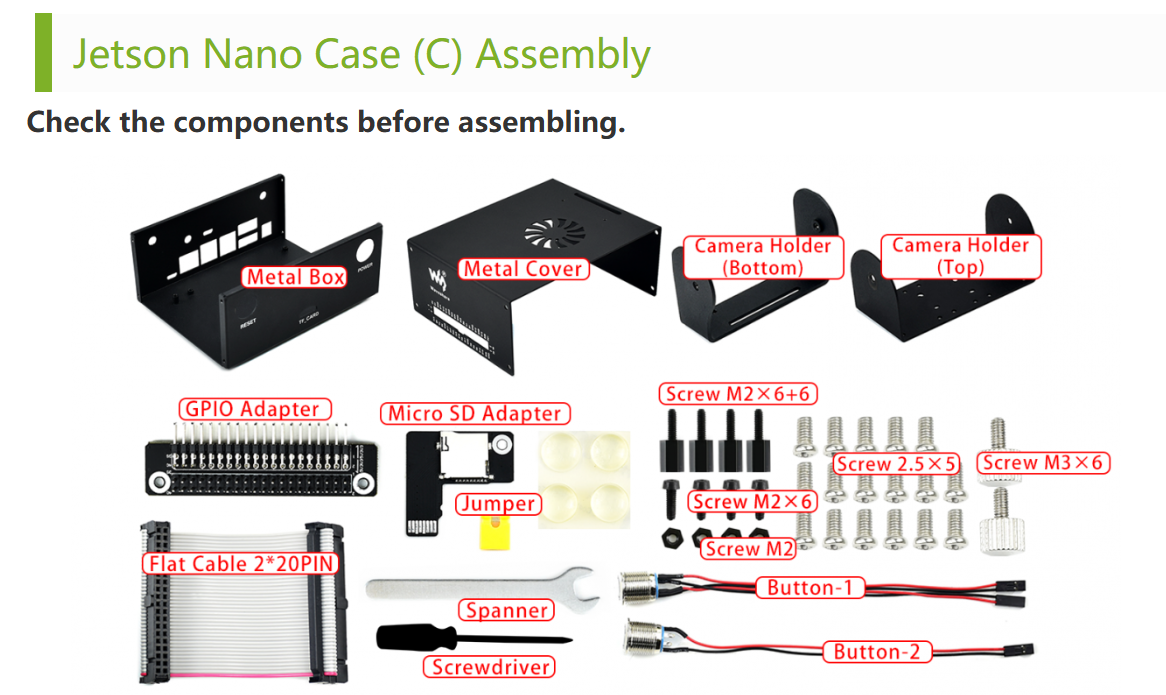
\includegraphics[width=0.9\linewidth]{../NVIDIAJetsonNano/images/WaveshareCase.png}
		\caption{Waveshare Case}
	\end{figure}
}

\STANDARD{NVIDIA Jetson Nano Developer Kit A02 model}
{
	NVIDIA Jetson Nano has 2 models in J1010 there are 2 Type C ports and in standard NVIDIA Jetson Nano consists of 1 Micro USB and 1 Type C port.\cite{NVIDIA:2020}		
	{
		\begin{figure}
			\centering
			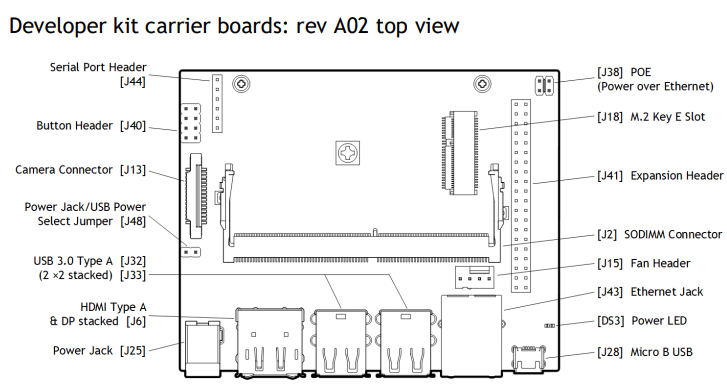
\includegraphics[width=0.7\linewidth]{../images/NVIDIAJetsonNanoA02TopView}
			\caption{NVIDIA Jetson Nano Developer Kit 2GB (original A02 model)}
		\end{figure}
	}
}

\STANDARD{Power and Reset Connections}
{
\begin{figure}
	\centering
	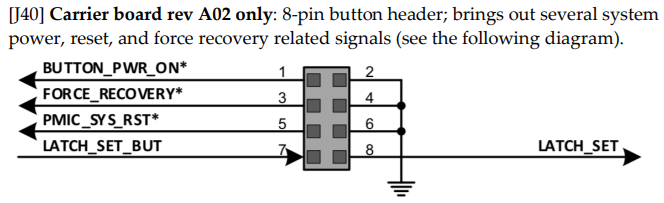
\includegraphics[width=0.7\linewidth]{images/HeaderPin}
	\caption{[J40] Header Pins of NVIDIA Jetson Nano Developer Kit A02 model}
\end{figure}
	\begin{itemize}
		\item Pins 7 and 8 disable auto power-on.
		\item Pins 1 and 2 initiate power-on if auto power-on is disabled.
		\item Pins 5 and 6 reset the system.
	\end{itemize}
	\begin{figure}
		\centering
		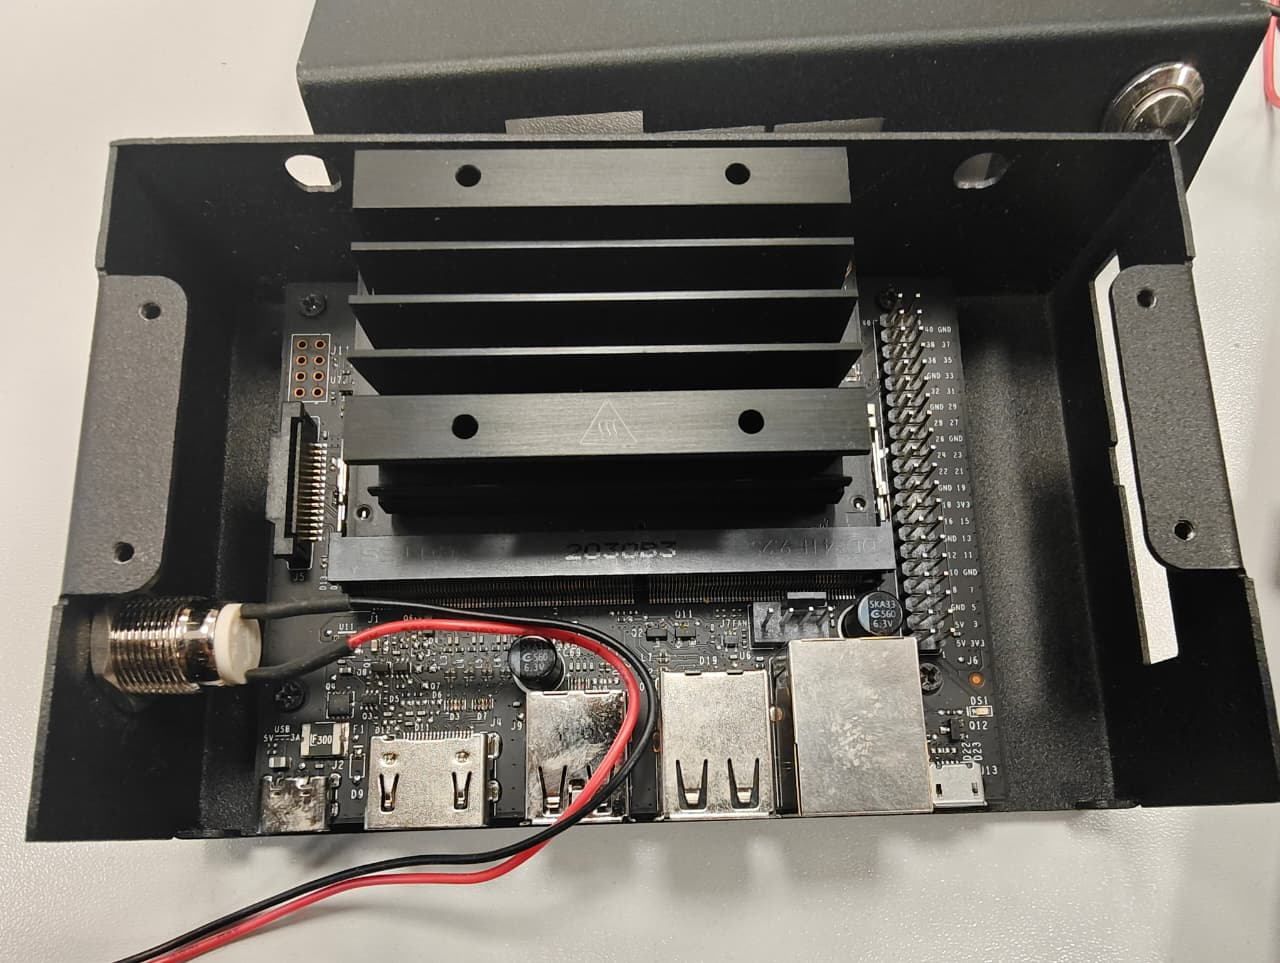
\includegraphics[width=0.7\linewidth]{../images/NVIDIAJetsonNanoinWaveshareCase}
		\caption{NVIDIA Jetson Nano Developer Kit A02 model inside Waveshare Case}
	\end{figure}
	[J41] 40-pin expansion header includes:
	\begin{itemize}
	
	\item Power pins.
	Two 3.3V power pins and two 5V power pins. These are not switchable; power is
	always available when the developer kit is connected to power.
	Two 5V pins can be used to power the developer kit at 2.5A each.
	\item Interface signal pins, All signals use 3.3V levels.
	\item By default, all interface signal pins are configured as GPIOs, except pins 3 and 5
	and pins 27 and 28, which are I\textsuperscript{2}C SDA and SCL, and pins 8 and 10, which are
	UART TX and RX. L4T includes a Python library, \PYTHON{Jetson.GPIO}, for controlling
	GPIOs.  \cite{NVIDIA:2020}	
	\end{itemize}
}
\STANDARD{NVIDIA Jetson Nano Developer Kit (Rev A02)— Interface}
{
	\begin{figure}
		\centering
		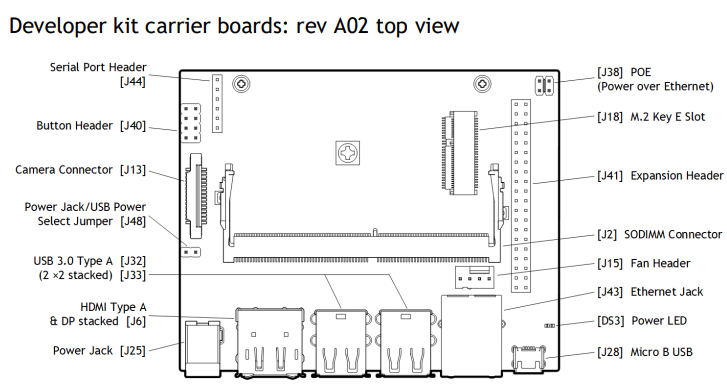
\includegraphics[width=\linewidth]{../images/NVIDIAJetsonNanoA02TopView}
	\end{figure}
	\begin{itemize}
		\item [J501] Slot for a microSD card.
		\item [Heatsink] Passive heatsink supporting 10W module power at 25°C ambient.
		\item [DS3] Power LED indicating system power-on.
		\item [J2] SO-DIMM connector for Jetson Nano module.
		\item [J6] HDMI and DisplayPort connector stack.
		\item [J13] Camera connector (CSI), supports IMX219 modules.
		\item [J15] 4-pin fan control header with PWM and tachometer support.
		\item [J18] M.2 Key E slot with PCIe x1, USB 2.0, UART, I2S, and I2C.
		\item [J25] 5V 4A barrel jack power input (2.1×5.5×9.5mm plug).
		\item [J28] Micro-USB 2.0 for 5V 2A power input or Device Mode.
		\item [J32] USB 3.0 Type A (two stacked).
		\item [J33] USB 3.0 Type A (two stacked).
		\item [J38] Power over Ethernet header exposing DC voltage from RJ45.
		\item [J40] 8-pin button header for power, reset, force recovery.
		\item [J41] 40-pin expansion header with 3.3V signals and power pins.
		\item [J43] RJ45 Gigabit Ethernet connector.
		\item [J44] 3.3V serial port header (UART console).
		\item [J48] Power select jumper for choosing J28 or J25 as power source.
	\end{itemize}
}


\Mysection{Next Steps}
\STANDARD{Next Steps on NVIDIA Jetson Nano Developer Kit}
{
	\begin{itemize}
		\item Note the tests that are successful 
		\item Check for version of Jetpack and document it.
		\item Calibrate the External Sensors and components based on the requirements of project.
		\item Camera used in this project 
		\item JetBot is an open-source AI project for makers, students and enthusiasts who are interested in learning AI and building fun applications. JetBot is a great launchpad for creating entirely new AI projects. \cite{NVIDIA:2020}	
	\end{itemize}
}